\documentclass[12pt, twoside]{article}
\usepackage[letterpaper, margin=1in]{geometry}
\usepackage[english]{babel}
\usepackage[utf8]{inputenc}
\usepackage{amsmath}
\usepackage{amsfonts}
\usepackage{amssymb}
\usepackage{tikz}
\usepackage{venndiagram}
\usepackage{multicol}

\usepackage{fancyhdr}
\pagestyle{fancy}
\fancyhf{}
\renewcommand{\headrulewidth}{0pt} % disable the underline of the header

\fancyhead[RE]{\thepage}
\fancyhead[RO]{\thepage \\ Name: \hspace{3cm}}
\fancyhead[L]{BECA / Dr. Huson / IB Math\\* 6 September 2019}


\begin{document}
\subsubsection*{Homework: Graphing and algebra review}
Simplify by collecting like terms.

  \begin{enumerate}

\item $2x^2+13x -12 -2x^2-3x+5$ \vspace{3cm}
\item $3(a^2-2a +7) -2(a^2-3a-10)$ \vspace{5cm}
\item $(a +7)(3a-1)$ \vspace{3cm}


Solve for the value of $x$.
\item   $-9= \frac{3}{4}x$ \vspace{3cm}
\item   $\frac{2}{3}(3x-6)=-2x$ \vspace{3cm}

\newpage
What is the slope and $y$-intercept of each equation?
  \begin{multicols}{2}
    \item   $y=-3.4x-1.8$
    \item   $5x+2y=8$
  \end{multicols} \vspace{3cm}

Use pencil for graphs. Label each function with its name or equation.
\item Given the function $f(x)=\frac{2}{5}x-5$.
\begin{enumerate}
    \item Draw the function $f(x)$ on the graph below.
    \item Mark and label the point $P (3, 2)$ on the graph.
    \item A second line, $g(x)$, is perpendicular to $f(x)$ and passes through point $P$. Plot $g(x)$ on the graph.
    \item Challenge: what is the exact value of the $y$-intercept of $g(x)$?
\end{enumerate}

\begin{figure}[!ht]
    \centering
    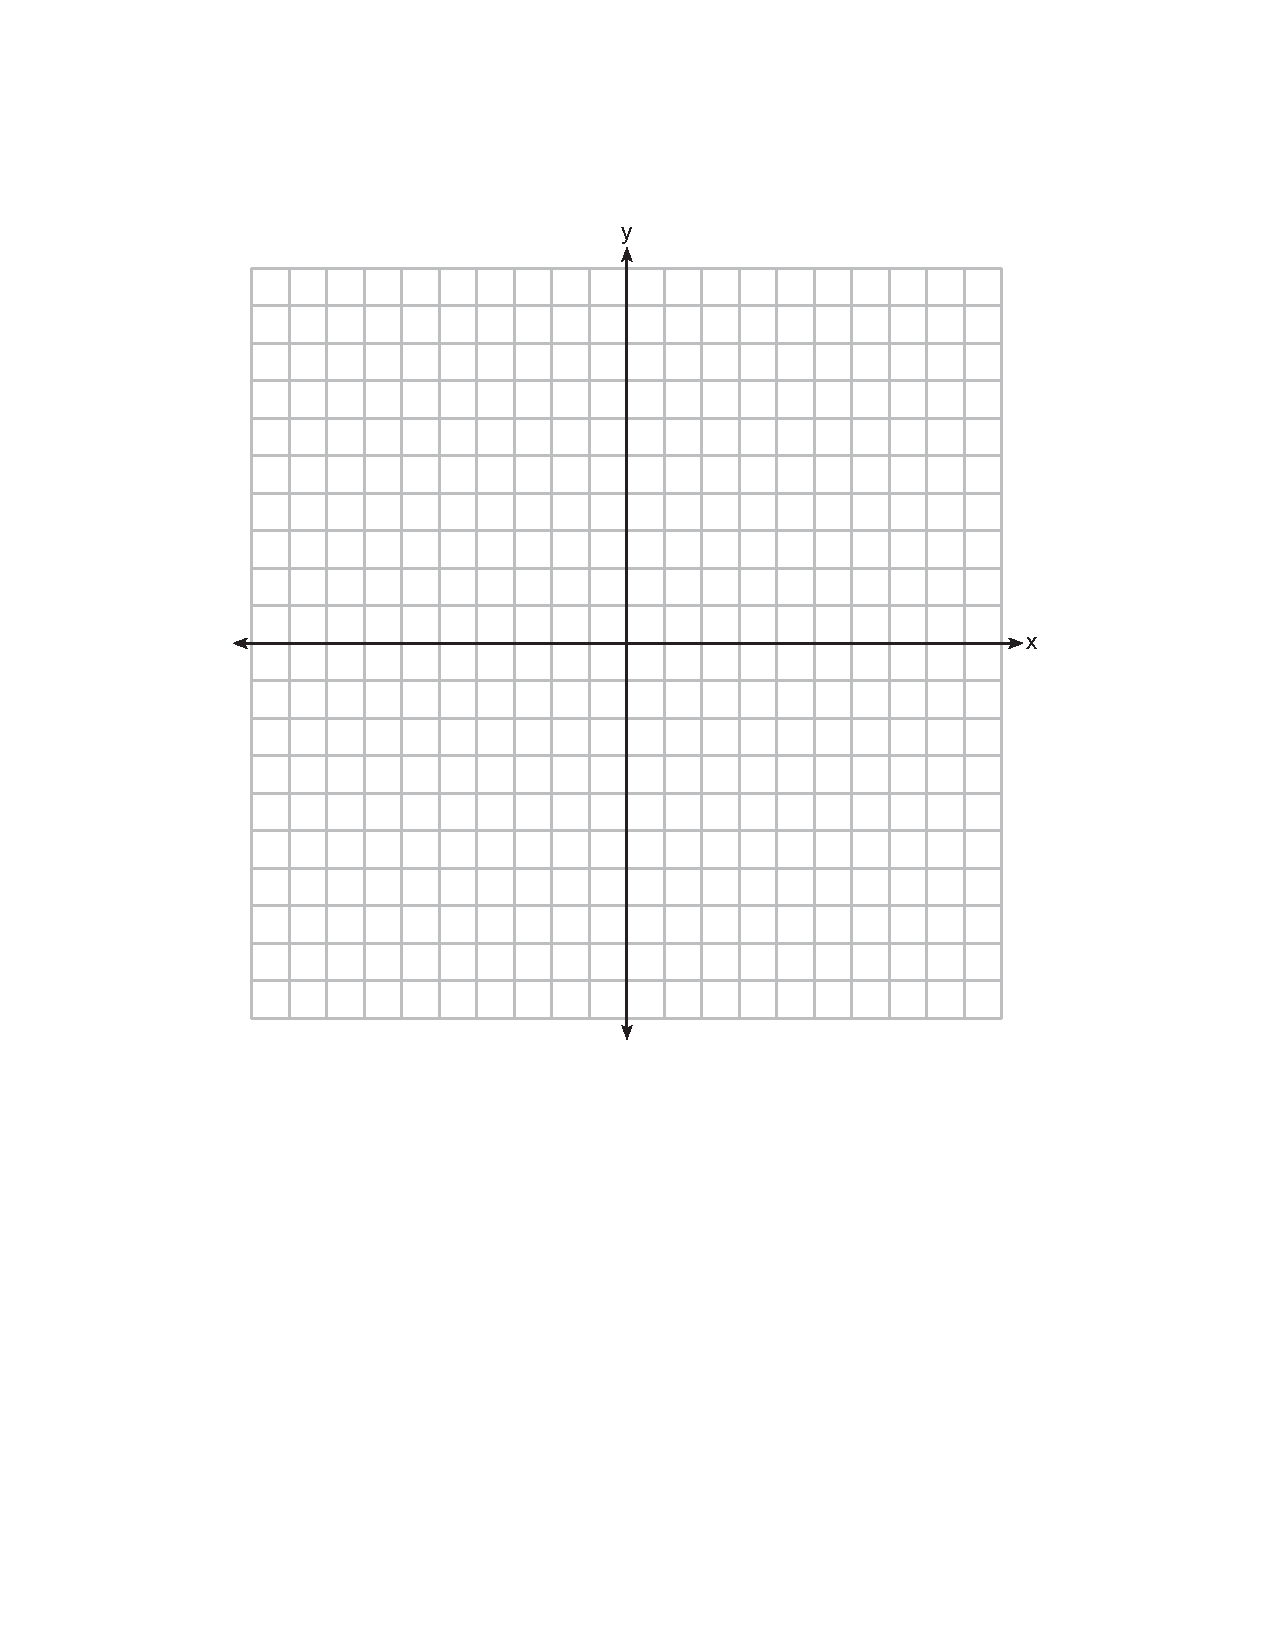
\includegraphics[width=0.65\textwidth]{regents-grid.pdf}
\end{figure}

\newpage

\item Explain why the radical $\sqrt[3]{5^2}$ is equivalent to $25^{\frac{1}{3}}$, an expression with a rational exponent. \vspace{4cm}

\item Solve the system of equations by graphing. Select a point in the solution set and label it on the graph as ordered pair.
\[x+4y \geq -8\]
\[y < \frac{1}{2}x-4\]

\begin{figure}[!ht]
    \centering
    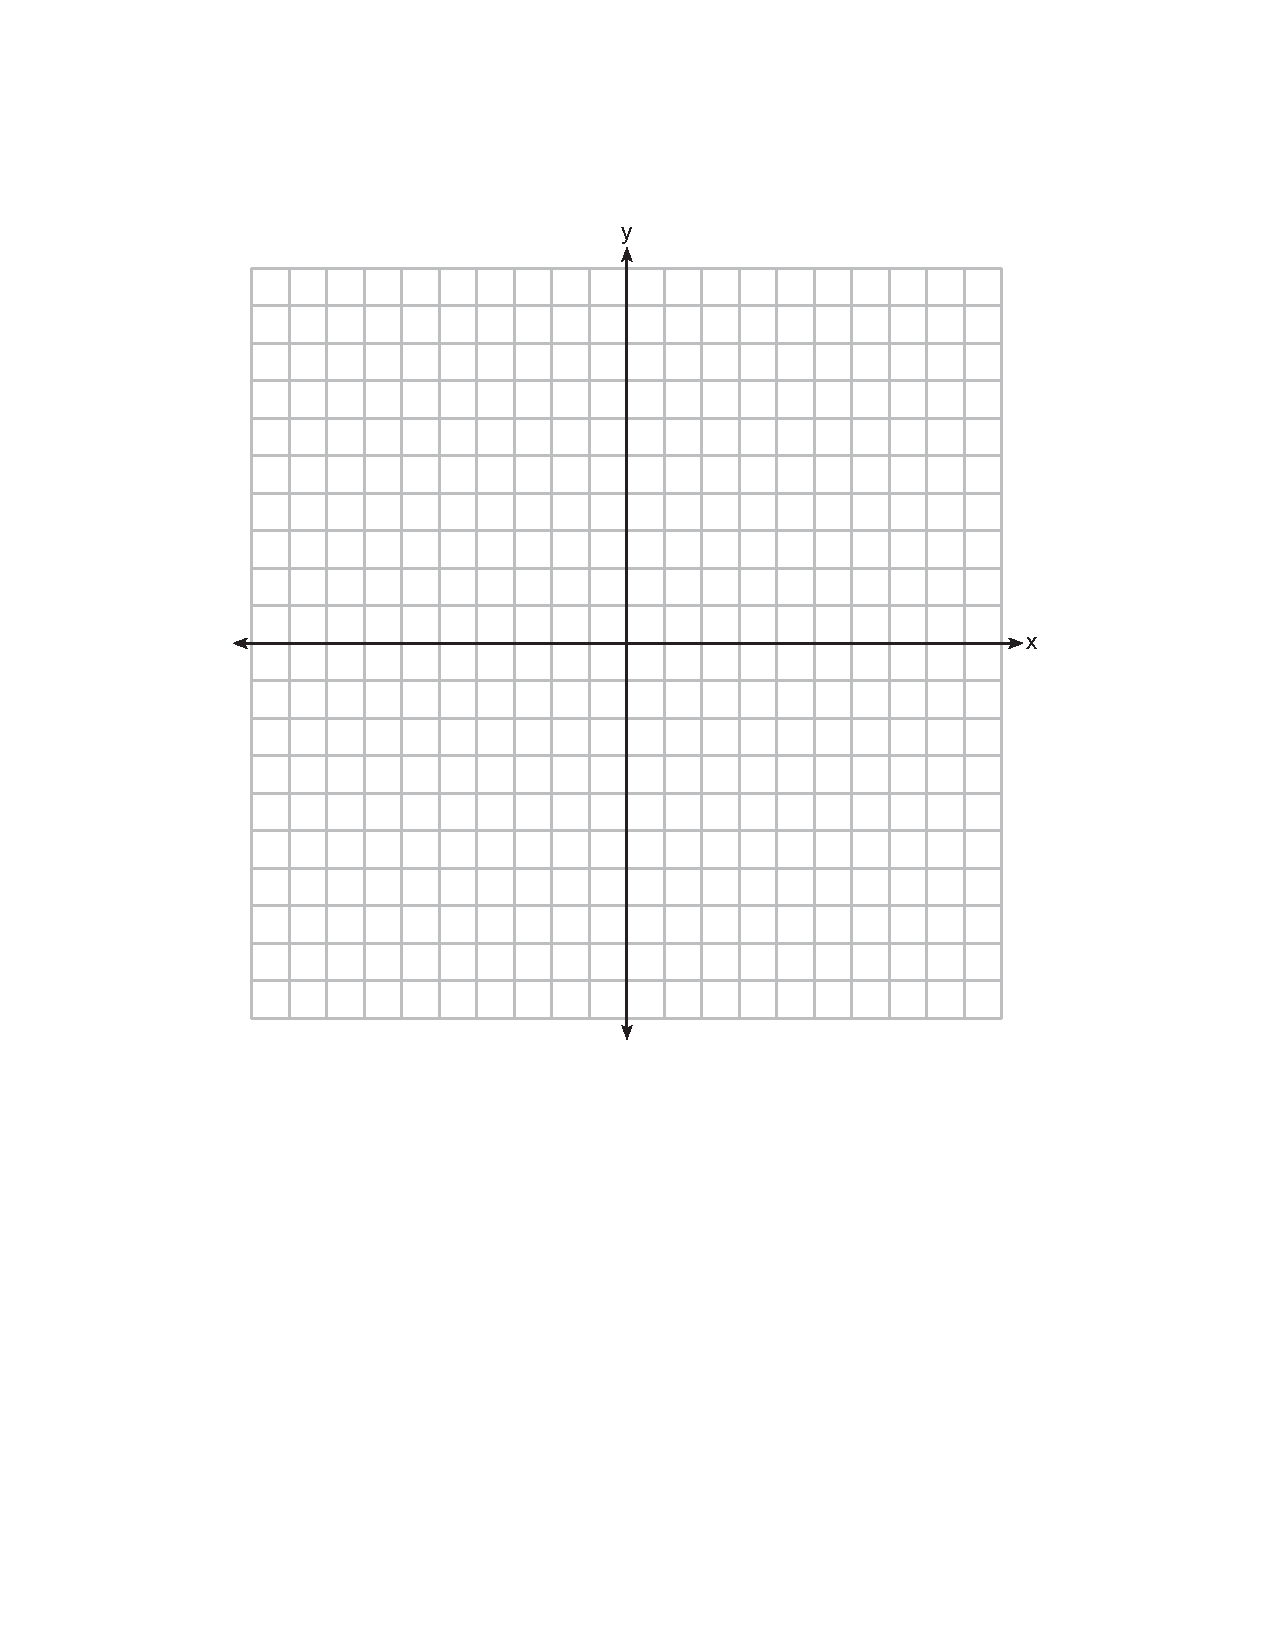
\includegraphics[width=0.65\textwidth]{regents-grid.pdf}
\end{figure}

\newpage
\item Graph the function $f(x)=x^2-x-12$ over the domain $-4 \leq x \leq 5$. Label the intercepts, axis of symmetry (with its equation), and the vertex as an coordinate pair.

    \begin{figure}[!ht]
        \centering
        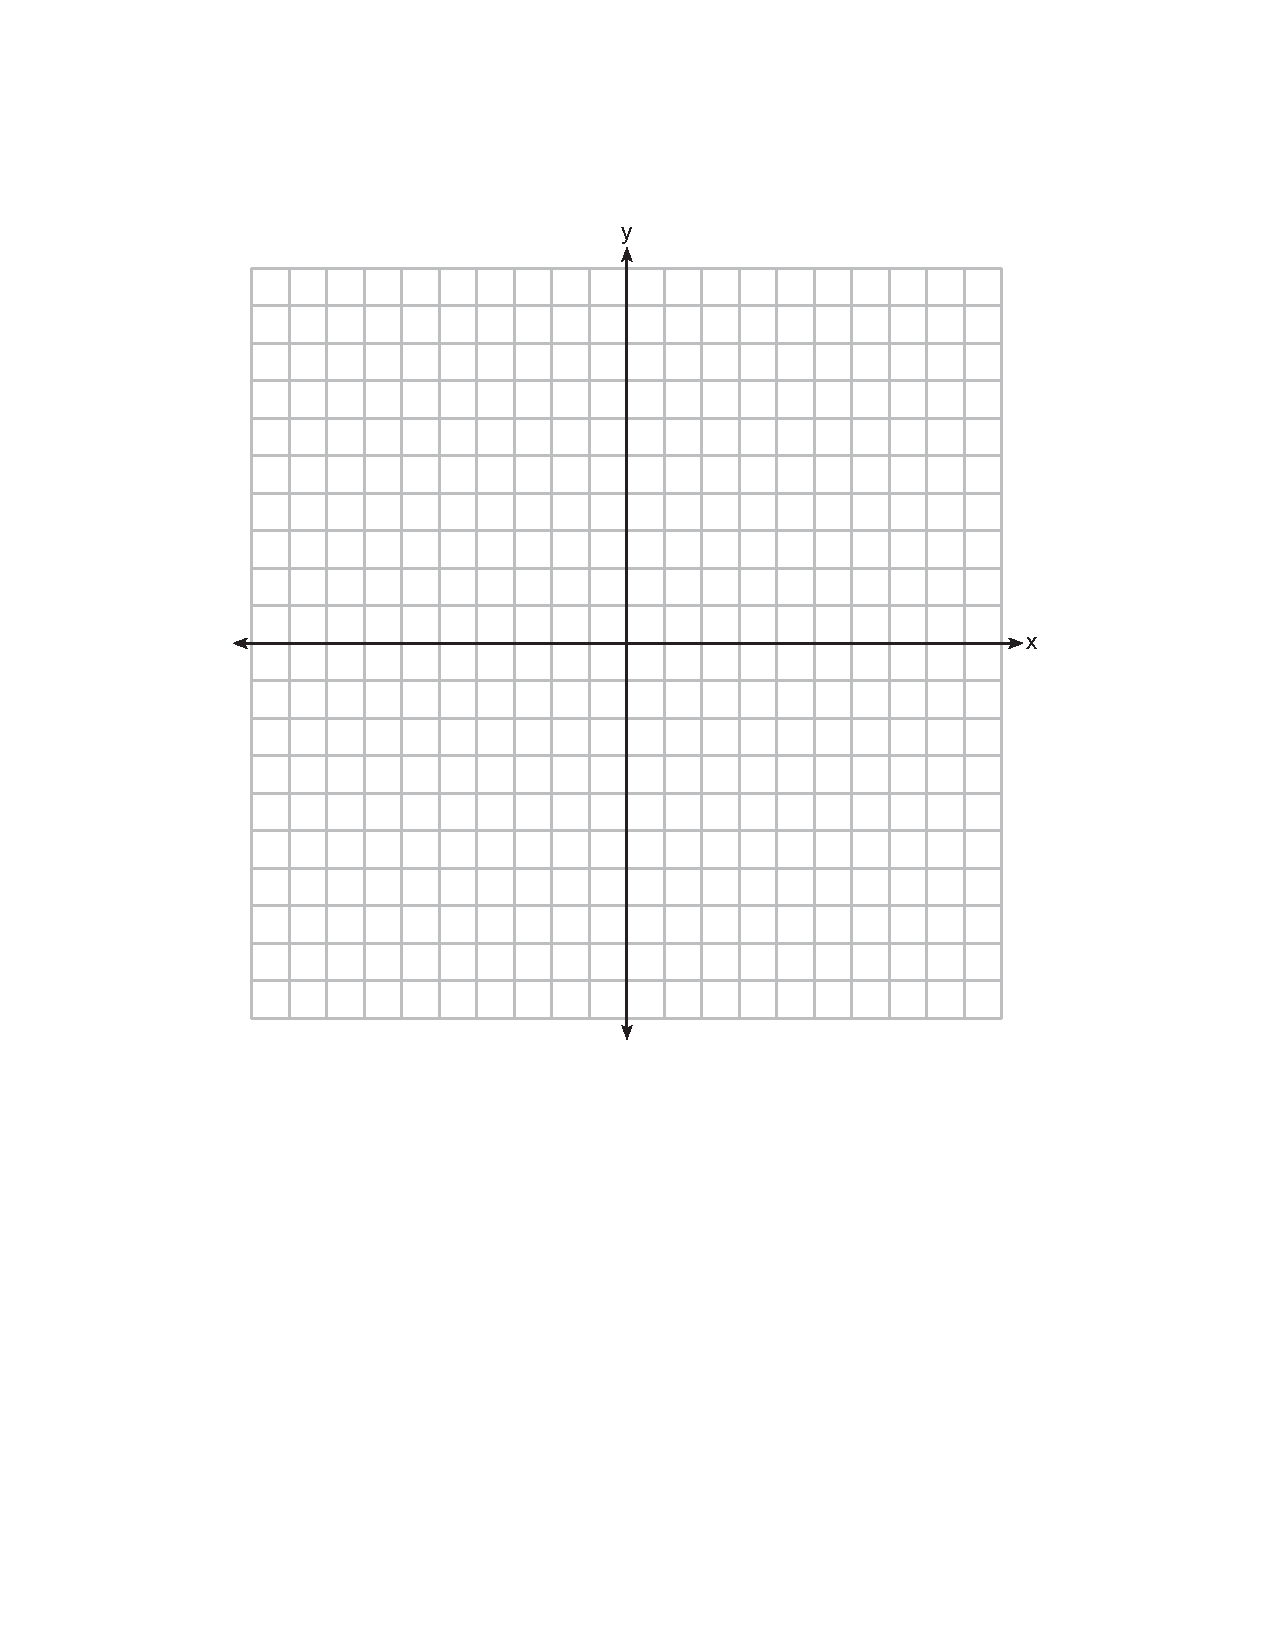
\includegraphics[width=0.75\textwidth]{regents-grid.pdf}
  \end{figure}

Solve the system algebraically.
\item
$3x+4y=15$\\*
$3x+y=3$


\end{enumerate}

\end{document}
